\documentclass{article}

% mathematical typesetting
\usepackage[]{amsmath} 
\usepackage[]{amsthm} 
\usepackage[]{amssymb} 

% lists
\usepackage[]{enumerate} 

% bibliography management
\usepackage[backend=biber, style=alphabetic]{biblatex} 
\addbibresource{../bib/mat2000.bib}

% index management
\usepackage[]{makeidx} 
\makeindex

% cross-references
\usepackage[]{hyperref} 
\usepackage[]{cleveref} 

% image handling
\usepackage[]{graphicx} 

% proclamation definitions
\theoremstyle{definition}
\newtheorem{defn}{Definition}
\newtheorem{exm}{Example}
\theoremstyle{plain}
\newtheorem{thm}{Theorem}
\newtheorem{lma}{Lemma}
\newtheorem{crl}{Corollary}
\newtheorem{prp}{Proposition}


% auxilliary commands
\newcommand{\proj}{\ensuremath{\mathbb{P}}} % projective space
\newcommand{\R}{\ensuremath{\mathbb{R}}}    % the real numbers
\newcommand{\projp}[3]{\ensuremath{[ #1 : #2 : #3 ]}}

\title{Visualizing Algebraic Surfaces}
\author{Ivar Haugal{\o}kken Stangeby}

\begin{document}

\begin{titlepage}

\maketitle

\begin{figure}[h!]
    \centering
    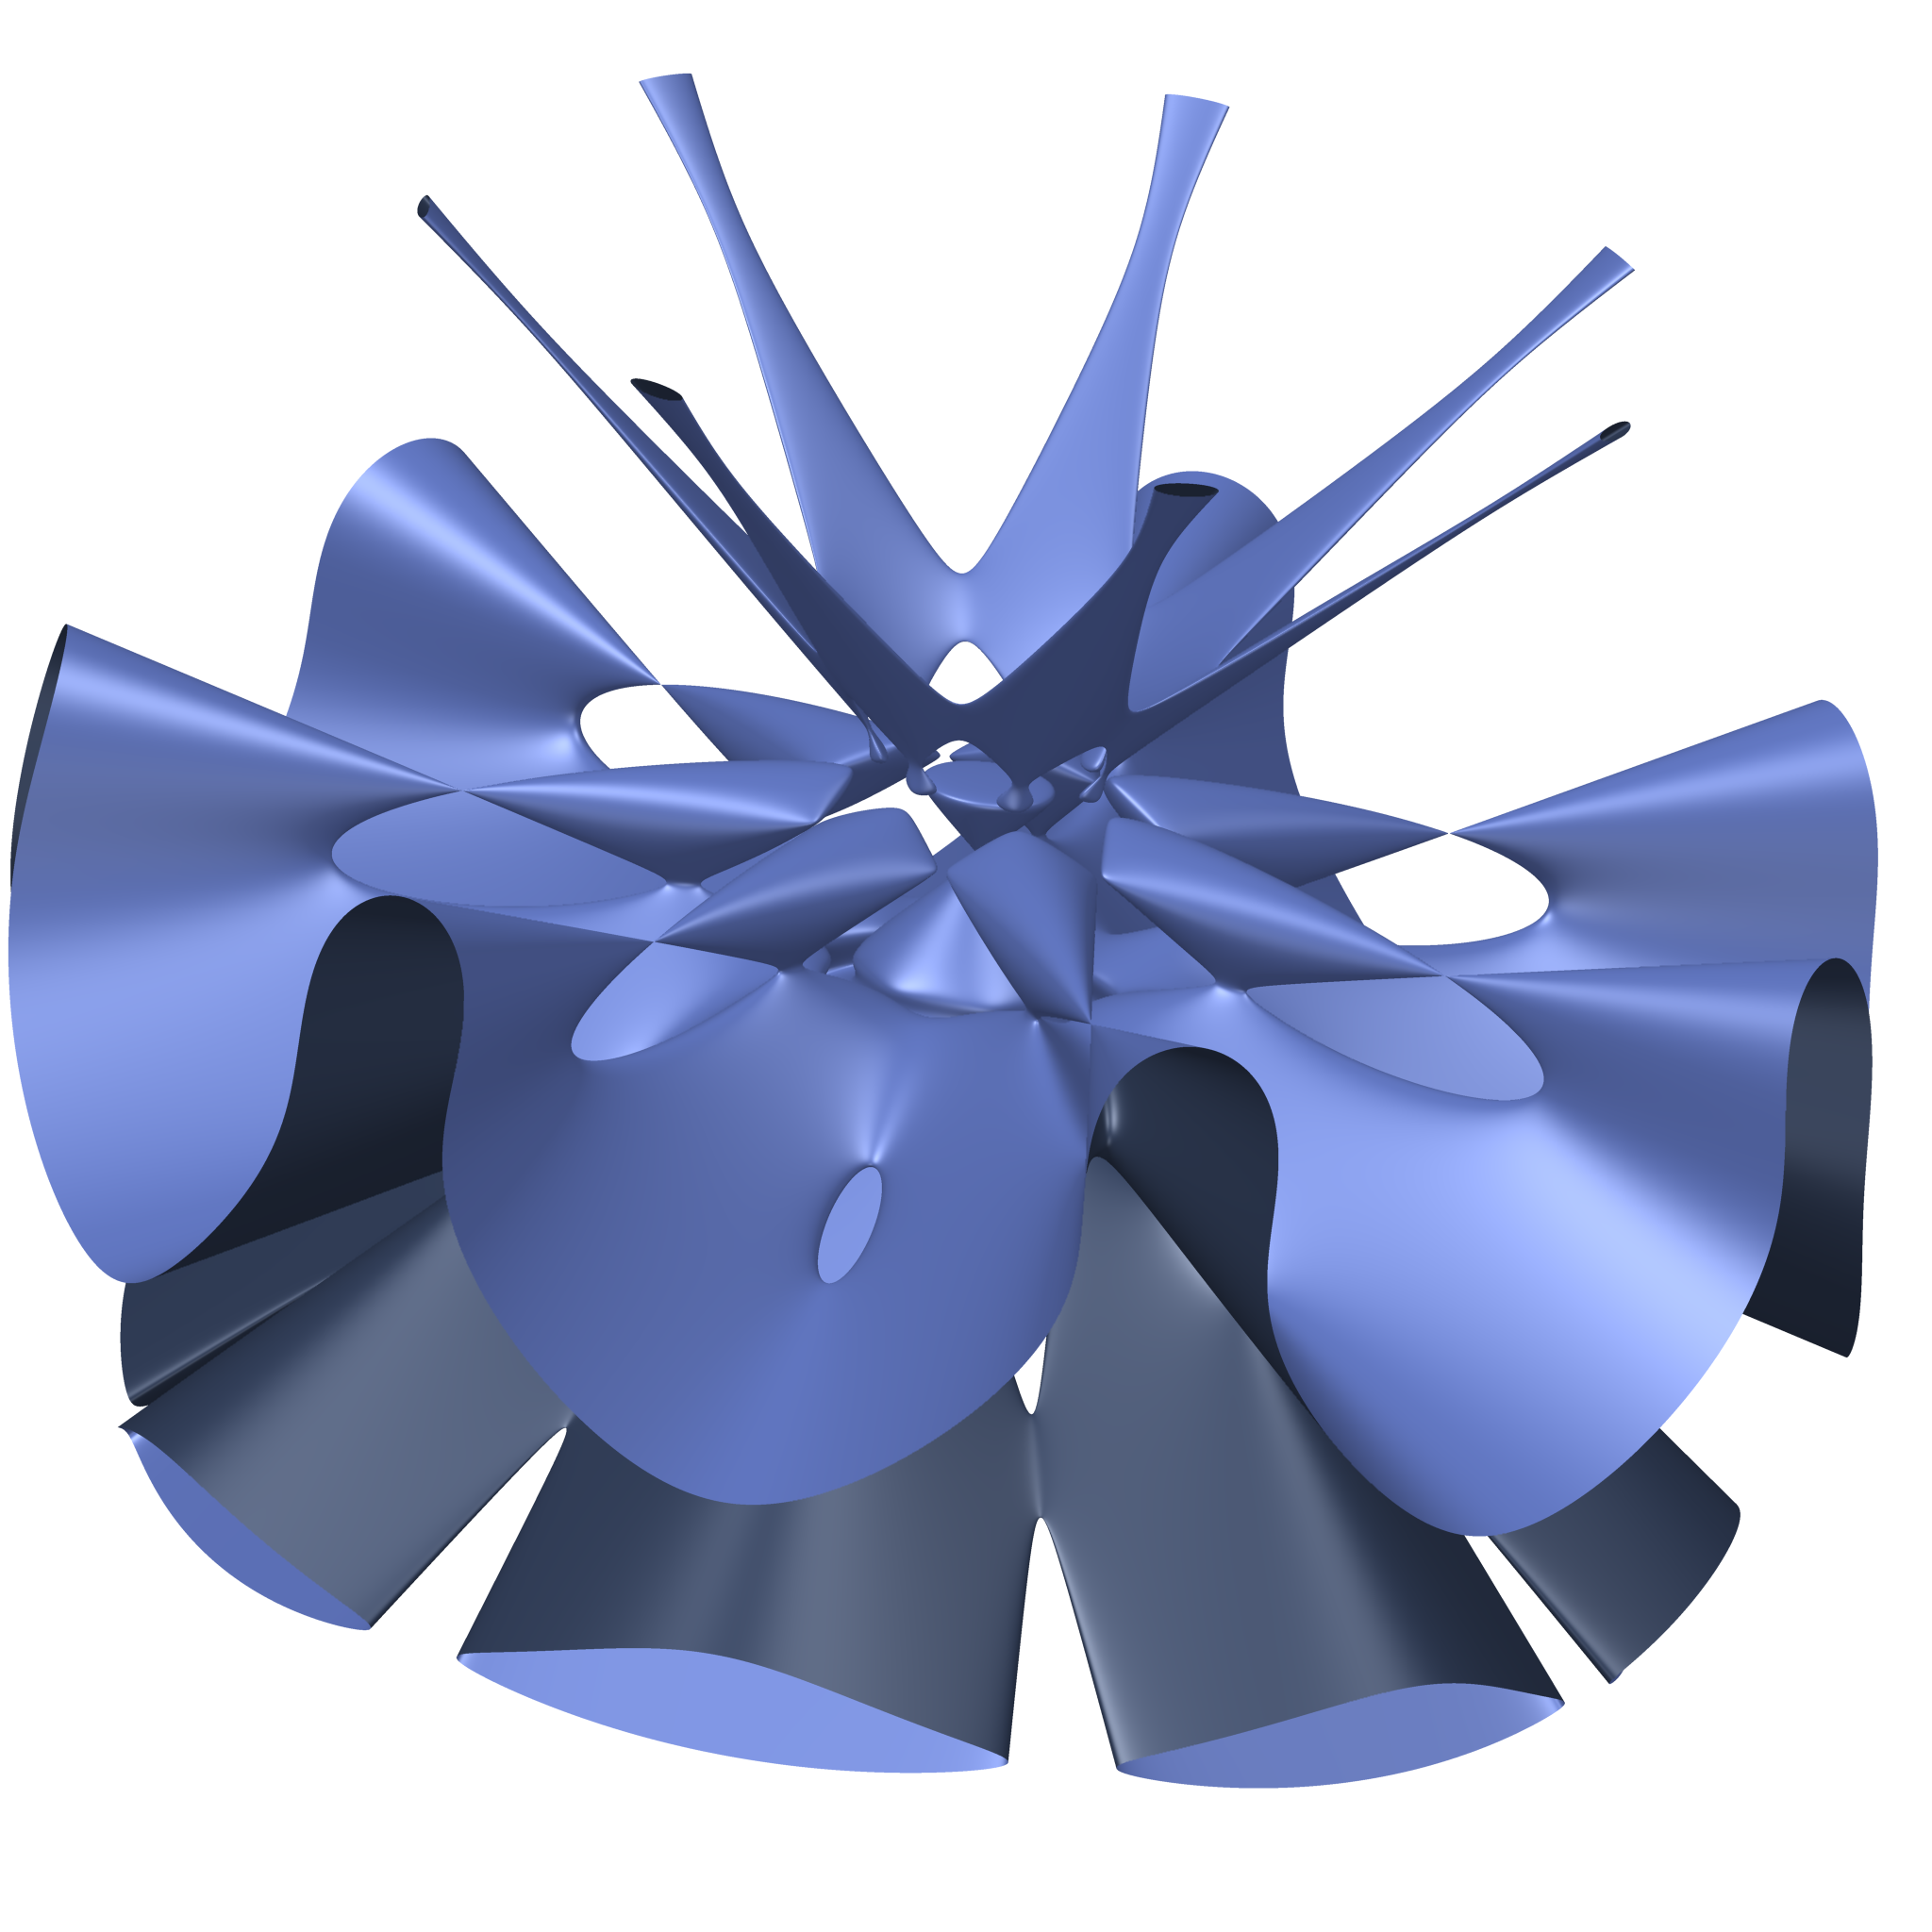
\includegraphics[width=0.8\linewidth]{../pictures/labs_septic.png}
\end{figure}

\end{titlepage}

\begin{abstract}
    
\end{abstract}

\tableofcontents

\section{Introduction}
\label{sec:introduction}

\section{Projective Space}
\label{sec:projective_space}

We start our study of algebraic surfaces by looking at \emph{projective space}.
Quite informally, projective space formalizes the notion of parallell lines
intersecting at infinity. In order to get a better understanding of the general
projective space $\proj^n$ we will first construct the \emph{real projective
plane}\index{real projective plane} $\proj^2(\R)$. 

\subsection{The real projective plane}
According to \cite{Wik16} there are three equivalent definitions:

\begin{enumerate}[I.]
    \item\label{def:one} The set of all lines in $\R^3$ passing through the origin $\left( 0,
        0, 0 \right)$. Every such line meets the \emph{sphere} of radius one
        centered in the origin exactly twice, say in $P = (x, y, z)$ and its
        antipodal point $(-x, -y, -z)$.
    \item\label{def:two} The points on the sphere $S^2$, where every point $P$ and its
        antipodal points are not distinguished. For example, the point $(1, 0,
        0)$ is identified with the point $(-1, 0, 0)$.
    \item The set of equivalence classes of $\R^3 \setminus \left\{(0, 0, 0)\right\}$ where
        two points $P$ and $P^\prime$ are considered equivalent if and only if
        there is a positive $\lambda \in \R$ such that $P = \lambda P^\prime$.
\end{enumerate}

The last definition is the one seemingly most commonly used, and is therefore
the one we will employ here. Note that the elements in the real projective
plane are equivalence classes of points in $\R^3$. We denote an element in
$\proj^2(\R)$ as $\projp{x}{y}{z}$. These elements are commonly referred to as
\emph{homogenous coordinates}\index{homogenous coordinates}. We state this
formally in a definition.

\begin{defn}[The real projective plane]
    Let $\sim$ be the equivalence relation on $\R^3$ defined by
    \begin{equation}
        \notag
        (x, y, z) \sim (x', y', z') \iff (x, y, z) = \lambda(x, y, z),
    \end{equation}
    where $\lambda$ is some positive real number. Then we denote the
    equivalence class of $(x, y, z)$ as $\projp{x}{y}{z}$ and we define
    \emph{the real projective plane} as the set
    \begin{equation}
        \notag
        \proj^2(\R) = \left\{ \projp{x}{y}{z} \mid (x, y, z) \in \R^3 \setminus
        \left\{ (0, 0, 0) \right\} \right\}.
    \end{equation}
\end{defn}

We can also look at a subset of $\proj^2(\R)$, namely the set of points
$\projp{x}{y}{z}$ where $z \neq 0$. Remembering the identification from the
above definition, these are equivalent to $\projp{\frac{x}{z}}{\frac{y}{z}}{1}$
with $\lambda = 1 / z$. If we consider definition \ref{def:two} from above,
this corresponds to the set of points on the northern hemisphere of $S^2$, not
including the circle of intersection in the $(x,y)$-plane. Similarly, we can
look at the set of points $\projp{x}{y}{0}$. This corresponds, in $S^2$, to the
circle of intersection in the $(x, y)$-plane. 

We can now take the notion of the projective plane and generalize to $n$
dimensions.
\subsection{Projective Space}
\label{sub:projective_space}

The general definition of projective $n$-space is completely anologous to the
definition of the projective plane, the set of lines in $\R^{n+1}$ passing
through the origin, however we include a formal definition for completeness.

\begin{defn}[The real projective space of dimension $n$]\index{projective space}
    Let $\sim$ be an equivalence relation on $\R^{n+1}\setminus \left\{ \left(
    0, \ldots, 0 \right) \right\}$ defined by
    \begin{equation}
        \notag
        \left( x_1, \ldots, x_{n+1} \right) \sim \left( x_1', \ldots, x_{n+1}' \right) 
        \iff \left( x_1, \ldots, x_{n+1} \right) = \lambda \left( x_1', \ldots, x_{n+1}' \right)
    \end{equation} 
    where $\lambda$ is some positive real number. We then denote the
    equivalence class of $\left( x_1, \ldots, x_{n+1} \right)$ by
    $\projp{x_1}{\ldots}{x_{n+1}}$ and define \emph{the real projective space
    of dimension $n$} as the set
    \begin{equation}
        \notag
        \proj^n(\R) = \left\{ \projp{x_1}{\ldots}{x_{n+1}} \mid \left( x_1, \ldots, x_{n+1} \right) \in \R^{n+1} \setminus \left\{ \left( 0, \ldots, 0 \right) \right\} \right\}.
    \end{equation}

\end{defn}

\section{Algebraic Surfaces}
\label{sec:algebraic_surfaces}

\printindex
\printbibliography

\end{document}
